\begin{center}
\textit{by N. Readioff, S. Olivares Pino, E. Petit, J. Stark, P. Bokan, D. Wardrope, M. Wielers}
\end{center}

A direct measurement of the Higgs boson trilinear self-coupling \lHHH can be made via the study of Higgs boson pair production. Only the dominant production mechanism at hadron colliders, gluon fusion, is considered, with the other production mechanisms being more than an order magnitude smaller.
The Feyman diagram which exhibits a \lHHH dependence interferes destructively with the box diagram that is independent of \lHHH , thus a small increase in the value of \lHHH decreases the expected HH production cross section, and modifies the distributions of event kinematics.

The small SM non-resonant HH production cross section means that it is necessary to consider final states where at least one of the two Higgs bosons decays into a final state with a large branching ratio, ie $H \rightarrow b\bar{b}$. The most promising decays channels are $HH \rightarrow b\bar{b}b\bar{b}$, $HH \rightarrow b\bar{b}\tau\tau$ and $HH \rightarrow b\bar{b}\gamma\gamma$ with branching ratios of 33.9, 7.3 and 0.26\% respectively.

%
\paragraph{The $HH \rightarrow b\bar{b}b\bar{b}$ channel}

Projections for this channel were made by extrapolating from the ATLAS Run 2 analysis of 24.3 $\ifb$ of 13~$\TeV$ data, described in Ref.~\cite{ITKPixelTDR}. This extrapolation assumes similar detector performance to Run~2. The largest source of systematic uncertainty comes from the ability to model the QCD multi-jet background using control regions in data. The allowed range at 95\% CL for $\kl$ including (without) systematic uncertainties is -4.1 -- 8.7 (-1.2 -- 8.0).

%
\paragraph{The $HH \rightarrow b\bar{b}\tau\tau$ channel}

Results~\cite{ATLASHHPUBnote} for this channel are computed by extrapolating from the Run 2 analysis of 36.1 $\ifb$ of 13~$\TeV$ data~\cite{ATLASrun2HHbbtautau}. A multivariate analysis with a boosted decision tree (BDT) is performed on the leptonic/hadronic and hadronic/hadronic decay modes of the $\tau$-lepton, and the BDT score is used as final discriminant. The largest systematic uncertainty of the Run 2 analysis, the simulation statistics, is neglected in the extrapolation. The expected significance of XX (XX) $\sigma$ including (without) systematics uncertainties can be achieved. The allowed range at 95\% CL for $\kl$ including (without) systematic uncertainties is XX -- XX (XX -- XX).


%
\paragraph{The $HH \rightarrow b\bar{b}\gamma\gamma$ channel}


The analysis~\cite{ATLASHHPUBnote} is based on truth level particles convoluted with the detector resolution, efficiencies and fake rates computed for $\mu$ = 200 which were extracted from fully simulated samples using the detector layout described in Ref.~\cite{ITKPixelTDR}. The selection is made using a multivariate analysis with a boosted decision tree. The diphoton invariant mass distribution, used to extract the signal through an analytical fit, is shown in Figure~\ref{fig:ATLAS_HH_a}. The number of signal, single Higgs and continuum background in a 123-127~$\GeV$ window is XX, XX and XX respectively, leading to a significance of XX (XX)$\sigma$ including (without) systematics uncertainties. The allowed range at 95\% CL for $\kl$ including (without) systematic uncertainties is XX -- XX (XX -- XX).


\begin{figure}[!htb]
\centering 
\subfloat[]{\label{fig:ATLAS_HH_a}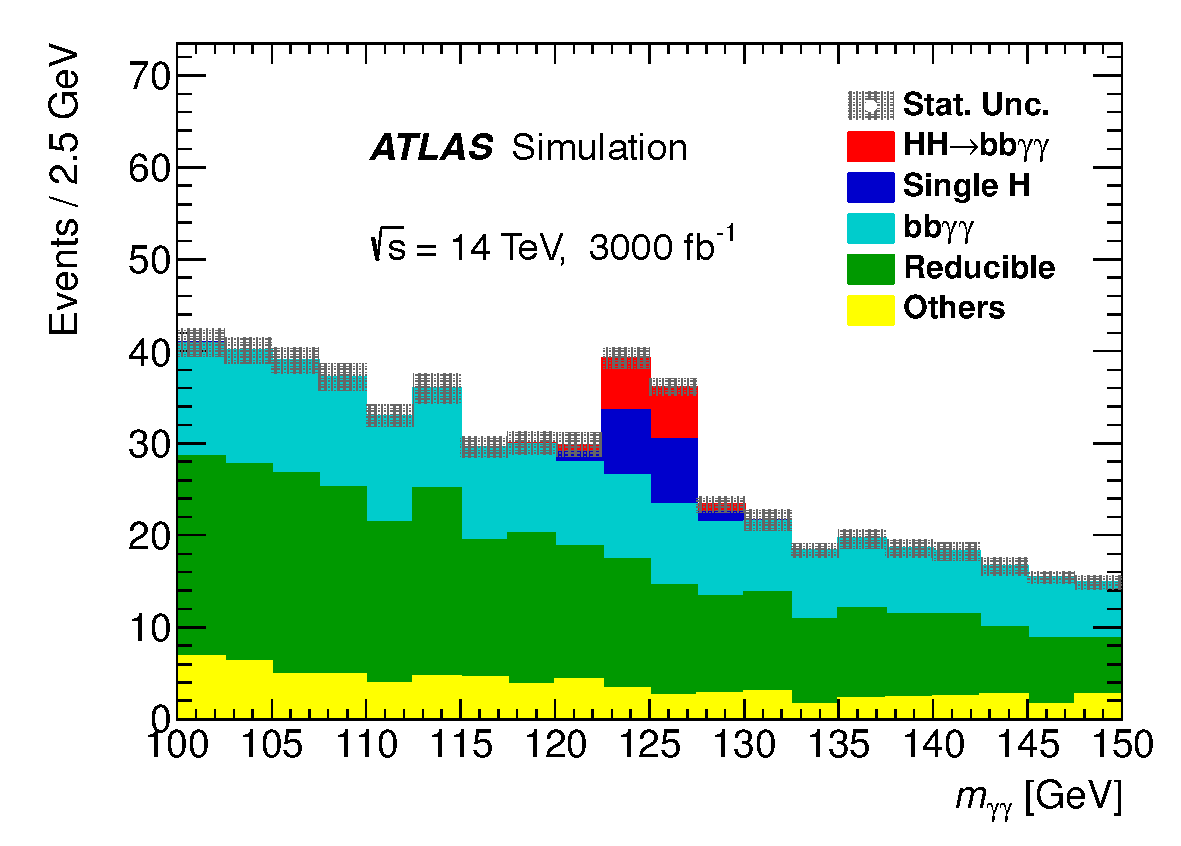
\includegraphics[width=0.5\textwidth]{section3/ch03_fig_033.pdf}} 
\subfloat[]{\label{fig:ATLAS_HH_b}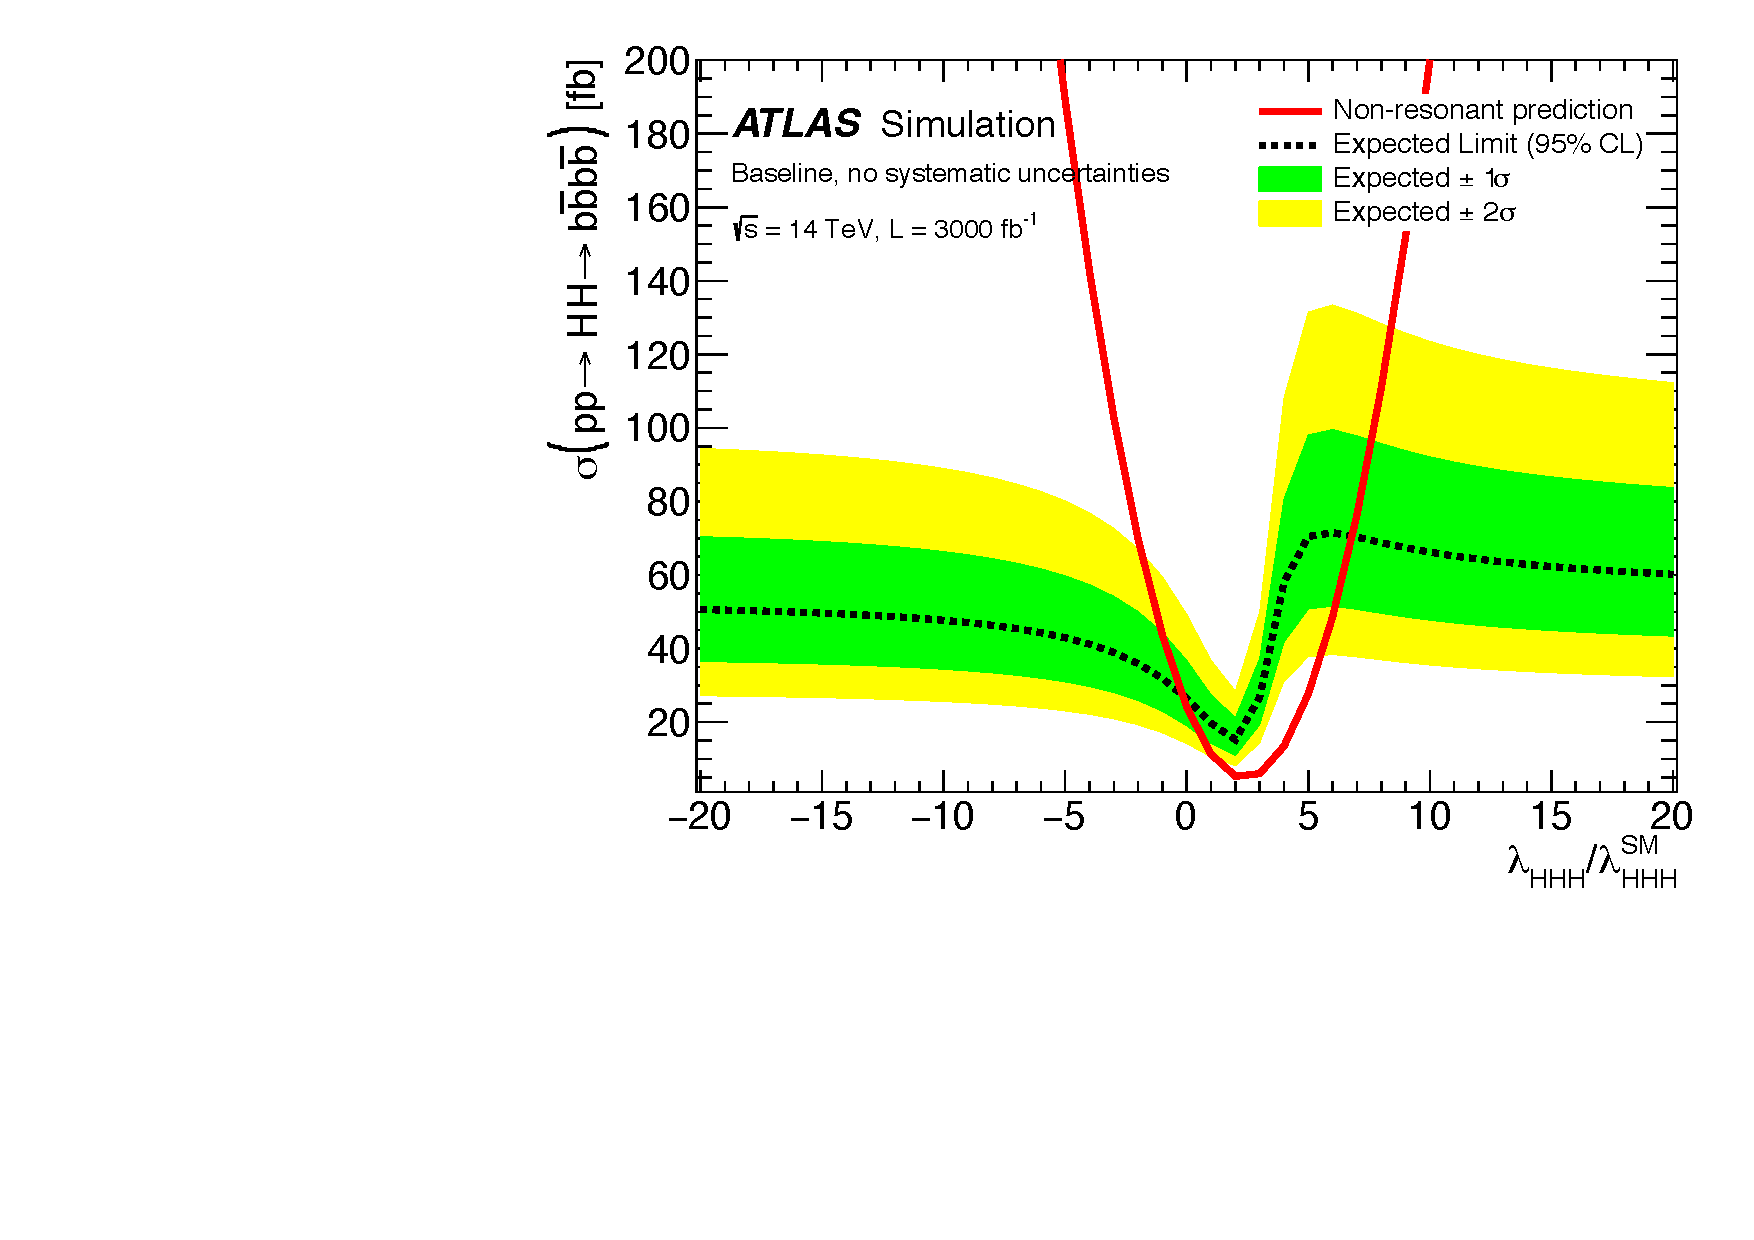
\includegraphics[width=0.5\textwidth]{section3/ch03_fig_035a.pdf}} 
\caption{(a)\textcolor{red}{PLACEHOLDER} Diphoton invariant mass distribution after selection, for the Standard Model HH signal and different background (plot from~\cite{ITKPixelTDR}). (b) \textcolor{red}{PLACEHOLDER} Expected 95\% CL upper limit on the cross-section $\sigma$(HH) with 3000 $\ifb$ of data, as a function of the Higgs self-coupling constant modifier \kl. The non-resonant HH prediction shows the theoretical cross-section for di-Higgs production as function of \kl\ (plot from~\cite{ITKPixelTDR}).} 
\label{fig:ATLAS_HH} 
\end{figure}


%
\paragraph{Combined results}

The combination of the three decay channels leads to an expected significance of XX (XX)$\sigma$ including (without) systematics uncertainties~\cite{ATLASHHPUBnote}. The 95\% CL upper limit on the HH production cross-section is shown in Figure~\ref{fig:ATLAS_HH_b}. The allowed range at 95\% CL for $\kl$ including (without) systematic uncertainties is XX -- XX (XX -- XX). A measurement of \lHHH\ is also performed, improved by the use of the $m_{HH}$ shape in the $HH \rightarrow b\bar{b}b\bar{b}$ and $HH \rightarrow b\bar{b}\gamma\gamma$ analyses. The trilinear coupling is measured to be:
%\begin{equation}
\[
\begin{split}
1^{+XX}_{-XX} [^{+XX}_{-XX} (stat) ^{+XX}_{-XX} (syst)] \text{ at 68\% CL} \\
1^{+XX}_{-XX} [^{+XX}_{-XX} (stat) ^{+XX}_{-XX} (syst)] \text{ at 95\% CL}
\end{split}
%\end{equation}
\]


